\documentclass[12pt]{article}

%%%  PACKAGES
\usepackage[utf8]{inputenc}
\usepackage{geometry}
\usepackage[frenchb]{babel}
\usepackage[T1]{fontenc}
\usepackage{array}           % for better arrays (eg matrices) in maths
\usepackage{subfig}			% make it possible to include more than one captioned figure/table in a single float
\usepackage{paralist}		% very flexible & customisable lists (eg. enumerate/itemize, etc.)
\usepackage{verbatim} 		% adds environment for commenting out blocks of text & for better verbatim
\usepackage{graphicx}		% Inclusion d'images-> \noindent\includegraphics[width=400px]{name}
\graphicspath{{images/}}		% le chemin ou aller chercher les graphics
\usepackage{listings}		% package for code listing
\usepackage{color}			% package to use color
\usepackage{hyperref}        % pour les liens cliquables (url, etc....)

%%%  PAGE DIMENSIONS
\geometry{a4paper} % or letterpaper (US) or a5paper or....
\geometry{a4paper, left=20mm, right=20mm, bottom=25mm, top=25mm}
\setlength{\parskip}{0.5em} % Espace entre les paragraphes

%%% USER COLORS
\definecolor{darkGreen}{RGB}{0,0.6,0}
\definecolor{gray}{RGB}{0.5,0.5,0.5}
\definecolor{mauve}{RGB}{0.58,0,0.82}
\definecolor{pblue}{rgb}{0.13,0.13,1}
\definecolor{pgreen}{rgb}{0,0.5,0}
\definecolor{pred}{rgb}{0.9,0,0}
\definecolor{pgrey}{rgb}{0.46,0.45,0.48}
\definecolor{red}{rgb}{1,0,0}
\definecolor{green}{rgb}{0,1,0}

%%% CODE STYLE (\lstinputlisting{stcFile.cpp} ou \begin{lstlisting} et \end{lstlisting}

%%% JAVA STYLE
\lstdefinestyle{Java}
{
  language=Java,
  inputencoding=utf8,
  frame=single,
  showspaces=false,
  showtabs=false,
  breaklines=true,
  showstringspaces=false,
  breakatwhitespace=true,
  commentstyle=\color{pgreen},
  keywordstyle=\color{pblue},
  stringstyle=\color{pred},
  basicstyle=\fontsize{9}{11}\ttfamily,
  numbers=left,
  numbersep=5px,
  numberstyle=\tiny\color{pgrey},
  stepnumber=1,
  tabsize=2,
}

%%% C++ STYLE
\lstdefinestyle{c++}
{
  language=C++,
  inputencoding=utf8,
  showtabs=false,
  breaklines=true,
  breakatwhitespace=true,
  stepnumber=1,
  basicstyle=\fontsize{9}{11}\ttfamily,
  commentstyle=\color{mygray},
  frame=single,
  numbers=left,
  numbersep=5px,
  numberstyle=\tiny\color{mygray},
  keywordstyle=\color{pblue},
  showspaces=false,
  showstringspaces=false,
  stringstyle=\color{myorange},
  tabsize=2
}

%%% XML Style
\lstdefinestyle{XML}
{
  inputencoding=utf8,
  language=XML,
  frame=lines,
  showspaces=false,
  showtabs=false,
  breaklines=true,
  showstringspaces=false,
  breakatwhitespace=true,
  commentstyle=\color{pgreen},
  keywordstyle=\color{pblue},
  stringstyle=\color{pred},
  basicstyle=\fontsize{9}{11}\ttfamily,
  numbers=left,
  numbersep=5px,
  numberstyle=\tiny\color{pgrey},
  stepnumber=1,
  tabsize=2
}

%%% JSON Style
\lstdefinestyle{JSON}
{
  inputencoding=utf8,
  frame=lines,
  showspaces=false,
  showtabs=false,
  breaklines=true,
  showstringspaces=false,
  breakatwhitespace=true,
  comment=[l]{:},
  commentstyle=\color{black},
  keywordstyle=\color{pblue},
  string=[s]{"}{"},
  stringstyle=\color{pblue},
  basicstyle=\fontsize{9}{11}\ttfamily,
  numbers=left,
  numbersep=5px,
  numberstyle=\tiny\color{pgrey},
  stepnumber=1,
  tabsize=2
}

%%% PHP Style
\lstdefinestyle{PHP}
{
  language=PHP,
  inputencoding=utf8,
  frame=lines,
  showspaces=false,
  showtabs=false,
  breaklines=true,
  showstringspaces=false,
  breakatwhitespace=true,
  comment=[l]{:},
  commentstyle=\color{black},
  keywordstyle=\color{pblue},
  string=[s]{"}{"},
  stringstyle=\color{pblue},
  basicstyle=\fontsize{9}{11}\ttfamily,
  numbers=left,
  numbersep=5px,
  numberstyle=\tiny\color{pgrey},
  stepnumber=1,
  tabsize=2
}

% Setup pour les liens
\hypersetup{
    bookmarks=true,         % show bookmarks bar?
    unicode=false,          % non-Latin characters in Acrobat’s bookmarks
    pdftoolbar=true,        % show Acrobat’s toolbar?
    pdfmenubar=true,        % show Acrobat’s menu?
    pdffitwindow=false,     % window fit to page when opened
    pdfstartview={FitH},    % fits the width of the page to the window
    pdftitle={My title},    % title
    pdfauthor={Author},     % author
    pdfnewwindow=true,      % links in new PDF window
    colorlinks=true,        % false: boxed links; true: colored links
    linkcolor=black,        % color of internal links (change box color with linkbordercolor)
    citecolor=green,        % color of links to bibliography
    filecolor=magenta,      % color of file links
    urlcolor=blue,          % color of external links
}

%%%  HEADERS & FOOTERS
\usepackage{fancyhdr}                   % This should be set AFTER setting up the page geometry
\pagestyle{fancy}                       % options: empty, plain , fancy
\renewcommand{\headrulewidth}{1pt}      % customise the layout...
\renewcommand{\footrulewidth}{1pt}
\lhead{
\includegraphics[width=50px]{logoheig2}}\chead{}\rhead{Projet IOT}
\lfoot{T. Besseau, M. Chatelan, L. Chauffoureaux, E. Schmid}\cfoot{}\rfoot{\thepage}

%%% SETTINGS %%%
\setlength\parindent{0pt} 		% Taille de l'indentation
\setcounter{tocdepth}{2}

%%% TITLE
\title{
  \vspace{-0.5cm}
  \huge{Projet IOT} \\
  \vspace{5mm}
  \Large{Analyse de menaces} \\
  \vspace{2.5cm}
  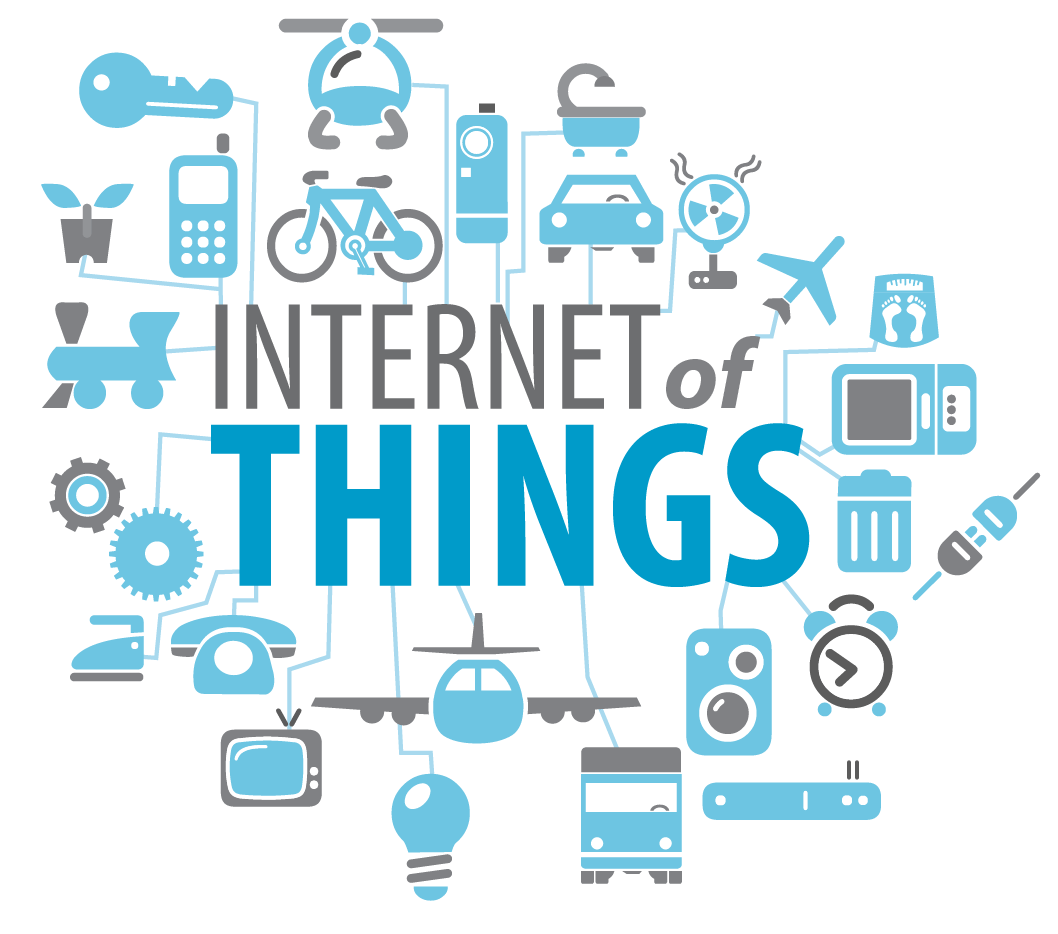
\includegraphics[width=.7\textwidth]{logo}
  \vspace{3cm}
}

\author{Thibaud Besseau, Matthieu Chatelan, Lara Chauffoureaux, Emmanuel Schmid}
\date{\today}

\begin{document}

\maketitle
\thispagestyle{empty}
\clearpage
\tableofcontents
\clearpage
\listoffigures
\clearpage
\headsep=20pt

\section{Introduction}
Ce document a pour but la sécurisation du projet élaboré dans le cadre du cours IoT dispensé à la HEIG-VD. Ce dernier est une plateforme de collecte de données environnementales issues de plusieurs capteurs. Dans ce document, les exigences du projet en général seront décrites ainsi que les biens nécessitant une protection contre tout type de menaces ou tout scénarios d'attaque ainsi que les contre-mesures associées. De plus, la liste de tous les composants hardware utilisés pour ce projet est donnée. Toutes les technologies utilisées pour ce projet ont été prises en compte.

\subsection{Equipes}
Lors de ce projet, nous avons créé 5 groupes distincts afin de répartir les différentes compétences et ainsi répartissant la charge de travail pour chacun de ces derniers. Chaucun des groupes avaient un répondant pour les autres groupes (représentés en gras ci-dessous).

\renewcommand{\arraystretch}{1.2}
\begin{center}
\begin{tabular}{|l|l|}
	\hline
	Groupe & Etudiant \\
	\hline
	Frontend & \textbf{Aurélie Lévy}  \\
	& Tony Clavien\\
	& Mathias Gilson\\
	\hline
	Backend & \textbf{Ludovic Delafontaine}   \\
	& Guillaume Milani\\
	& Sathiya Kirushnpillai\\
	& Mathieu Monteverde\\
	& Nicolas Rod\\
	\hline
	Sécurité & \textbf{Lara Chauffoureaux}  \\
	& Matthieu Chatelan  \\
	& Thibaud Besseau  \\
	& Emmanuel Schmid  \\
	\hline
	Firmware & \textbf{David Truan} \\
	& Théo Gallandat\\
	& Gaëtan Othenin-Girard\\
	& Marie Lemdjo\\
	& Ludovic Richard\\
	\hline
	Infrastructure & \textbf{Julien Brêchet} \\
	& Yosra Harbaoui\\
	& Guillaume Semeels\\
	& Adrien Marco\\
	& Ali Miladi\\
	& Dany Tchente\\
	\hline
\end{tabular}
\end{center}
\renewcommand{\arraystretch}{1}

\newpage
\section{Description du système}

\subsection{Objectifs du système}\label{objectifssysteme}% description précise du système (nb de capteurs, leur rôles, infra, ...)

Le but de ce système est la collecte de données depuis plusieurs capteurs répartis sur le site de Cheaseaux. Toutes les informations seront consultables sur un frontend accessible par les visiteurs authentifiés sur un compte publique.

Les différents capteurs (voir \autoref{elementssysteme}) se chargent de récolter des informations relatifs à leur environnement et les transmettent à une gateway dont le but est de collecter ces informations des différentes sources. Un bridge assure le lien entre le réseau LoRa et le réseau internet standard. Toutes les informations sont finalement transmises à un serveur d'applications sur lequel tourne le backend ainsi que le frontend.

Le schéma ci-dessous illustre cette architecture :

\begin{figure}[h!]
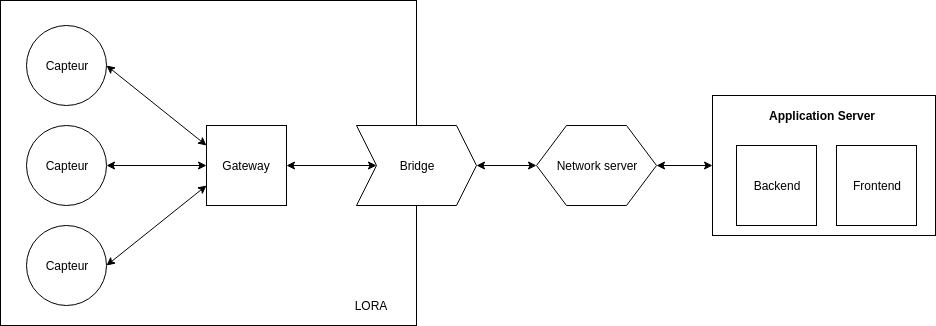
\includegraphics[width=\textwidth]{architecture}
\caption{Schéma de l'architecture du projet}
\end{figure}

\subsection{Exigences de l'application} % Ce qui est nécessaire pour que l'appli fonctionne + au niveau sécu

Pour la sécurité, nous avons interprété les exigences suivantes :

\begin{itemize}
\item[•] L'accès au backend ainsi que l'accès au frontend ne doit être possible que pour les personnes autorisées et authentifiées à l'aide d'un compte soit utilisateur, soit administrateur.
\item[•] Un utilisateur classique ne doit pas pouvoir accéder aux fonctionnalités réservées aux administrateurs.
\item[•] Les données transmises par les capteurs ne doivent pas être lisibles sur le réseau.
\end{itemize}

\newpage
\subsection{Éléments du systèmes}\label{elementssysteme} % Les différents capteurs, gateways, etc...

Afin de rendre ce système fonctionnel, plusieurs composants hardware ainsi que software doivent être utilisés. Les sous-sections suivantes représentent les différents modules hardware utilisés ainsi que les parties software développées pour ce projet.

\subsubsection{Capteurs}
La carte STM32 Nucleo (\autoref{nucleo}) offre aux utilisateurs un moyen abordable et flexible d'essayer de nouveaux concepts et de construire des prototypes avec le microcontrôleur STM32, en choisissant parmi les différentes combinaisons de performances, de consommation d'énergie et de fonctionnalités. Pour les cartes compatibles, le SMPS réduit considérablement la consommation d'énergie en mode Run.

Cette carte sera utilisée comme base pour tous les capteurs déployés dans le terrain.

\begin{figure}[!h]
	\centering
	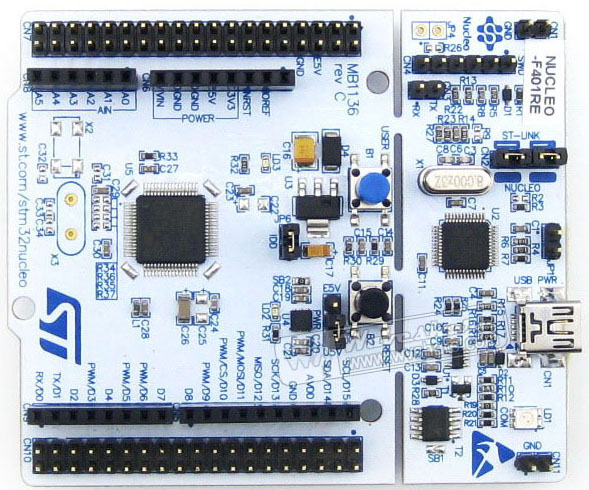
\includegraphics[width=350px]{nucleo}
	\caption{NUCLEO-F401RE}
	\label{nucleo}
\end{figure}

\newpage
Le shield utilisé pour ce projet (\autoref{shield}) rend un Arduino compatible avec plus de 75 capteurs de type clic. C'est un shield simple avec deux prises hôte mikroBUS ™ d'un côté et un connecteur Arduino à l'opposé.

\begin{figure}[!h]
	\centering
	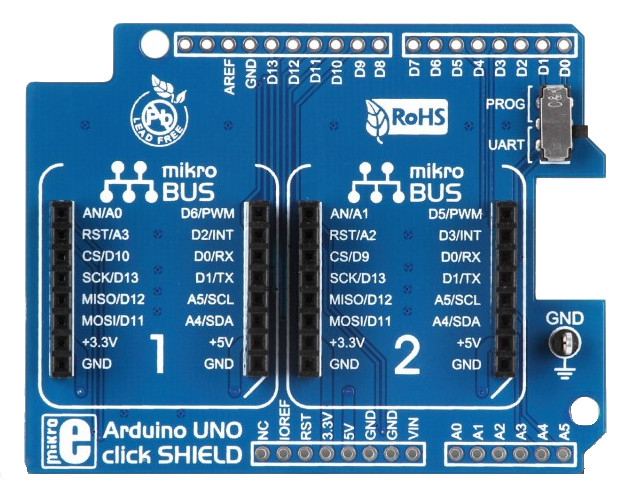
\includegraphics[width=250px]{shield}
	\caption{Arduino Uno Click Shield}
	\label{shield}
\end{figure}

Le module \textit{Environment click} (\autoref{ambient}) mesure la température, l'humidité relative, la pression et les COV (composés organiques volatils gazeux). Le clic intègre le capteur environnemental BME680 de Bosch. Environnement Click est conçu pour fonctionner sur une alimentation de 3,3 V. Il communique avec le microcontrôleur cible via l'interface SPI ou I2C.

\begin{figure}[!h]
	\centering
	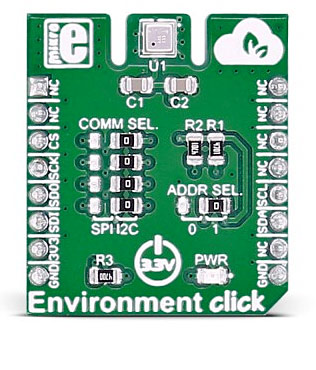
\includegraphics[width=200px]{ambient}
	\caption{Ambient 2 Click BME680}
	\label{ambient}
\end{figure}

\newpage
LoRaWAN ™ ou Low Area Wide Network est une technologie sans fil développée pour permettre des communications à bas débit sur de longues distances, principalement pour les applications IoT et les capteurs.

Le module émetteur-récepteur LoRa longue portée RN2483 de Microchip (\autoref{lora}) est une solution facile à utiliser et à faible consommation d'énergie pour la transmission de données sans fil à longue portée.

Le module RN2483 a une portée spécifiée> 15 km dans les zones rurales et suburbaines, et> 5 km dans les zones urbaines.

Une pile de protocole LoRaWAN ™ classe A est intégrée (périphériques finaux bidirectionnels), ainsi qu'une interface de commande ASCII accessible via UART. La sensibilité élevée du récepteur peut descendre à -148 dBm.
\begin{figure}[!h]
	\centering
	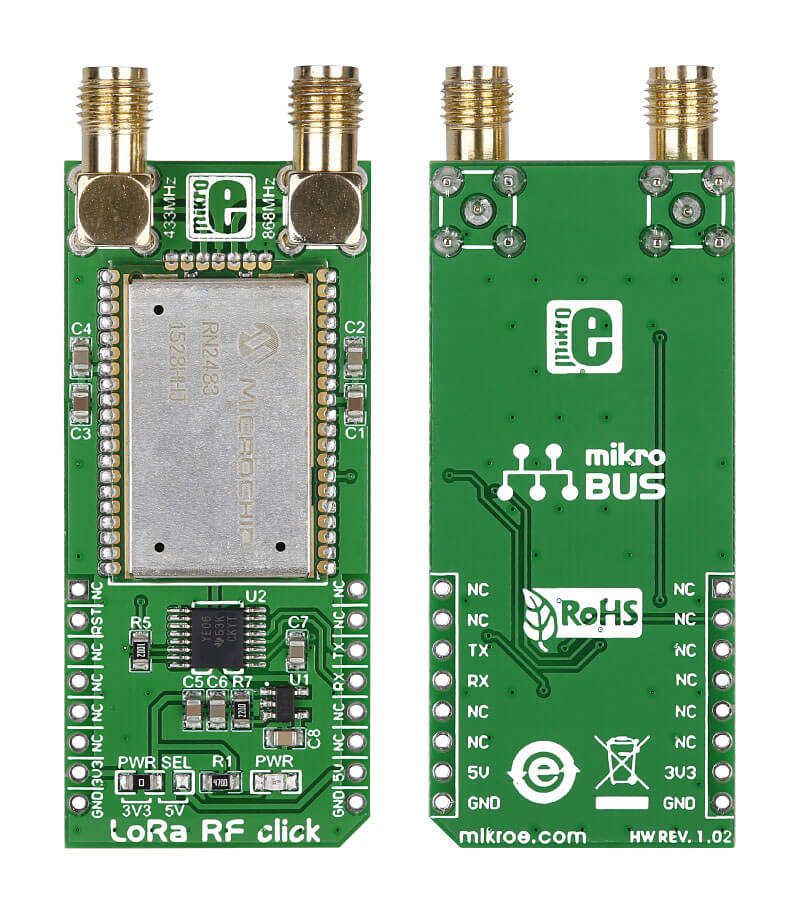
\includegraphics[width=150px]{lora}
	\caption{Lora Click}
	\label{lora}
\end{figure}

Ci-dessous, une photo du montage complet du capteur avec tous les modules attachés :
\begin{figure}[!h]
	\centering
	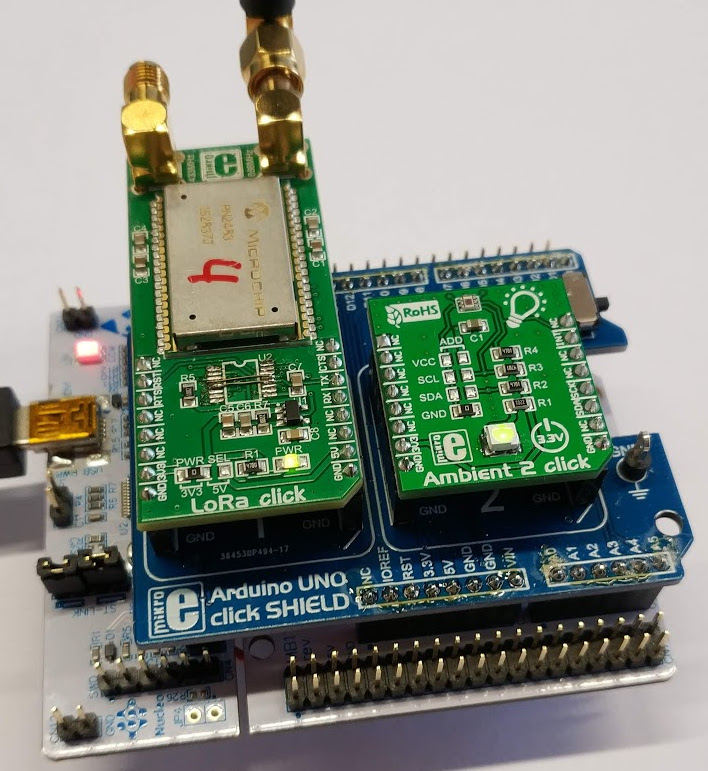
\includegraphics[width=200px]{montage}
	\caption{Montage complet du capteur}
	\label{}
\end{figure}

\newpage
\subsubsection{Gateway}

Le Raspberry Pi 2 Model B est le Raspberry Pi de deuxième génération. Il a remplacé l'original Raspberry Pi 1 Model B+ en février 2015.

Le Raspberry Pi 2 comporte les caractéristiques suivantes :

\begin{itemize}
	\item[•] 900MHz quad-core ARM Cortex-A7 CPU
	\item[•] 1GB RAM
	\item[•] 100 Base Ethernet
	\item[•] 4 Ports USB
	\item[•] 40 pins GPIO
	\item[•] Port HDMI
	\item[•] Jack audio 3.5mm et sortie vidéo composite
	\item[•] Interface Caméra (CSI)
	\item[•] Interface d'affichage (DSI)
	\item[•] Slot pour Micro SD
	\item[•] VideoCore IV 3D coeur graphique
\end{itemize}



\begin{figure}[!h]
	\centering
	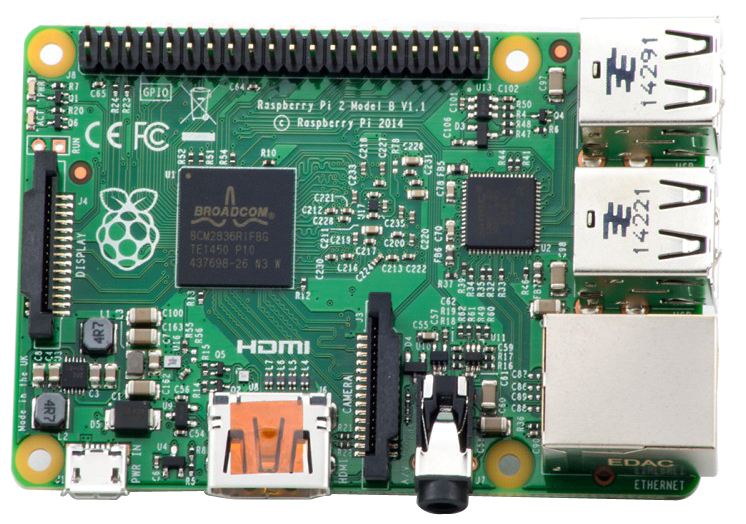
\includegraphics[width=350px]{raspberry}
	\caption{Raspberry Pi Model B}
	\label{raspberry}
\end{figure}

\newpage
Le module iC880A-SPI est capable de recevoir des paquets de différents appareils envoyés avec différents facteurs d'étalement sur jusqu'à 8 canaux en parallèle. En raison du fait que la combinaison des facteurs d'étalement et des largeurs de bande du signal donne des débits de données différents, l'utilisation de "Dynamic Data-Rate Adaption" devient possible. Cela signifie que les nœuds LoRa® à grande distance du concentrateur doivent utiliser des facteurs d'étalement plus élevés et donc avoir un débit de données plus faible.

Les nœuds LoRa qui sont plus proches du concentrateur peuvent utiliser des facteurs d'étalement plus faibles et peuvent donc augmenter leur débit de données. Cela permet de construire des réseaux étoiles ou multi-étoiles faciles à gérer sans besoin de routeurs ou de répéteurs.

\begin{figure}[!h]
	\centering
	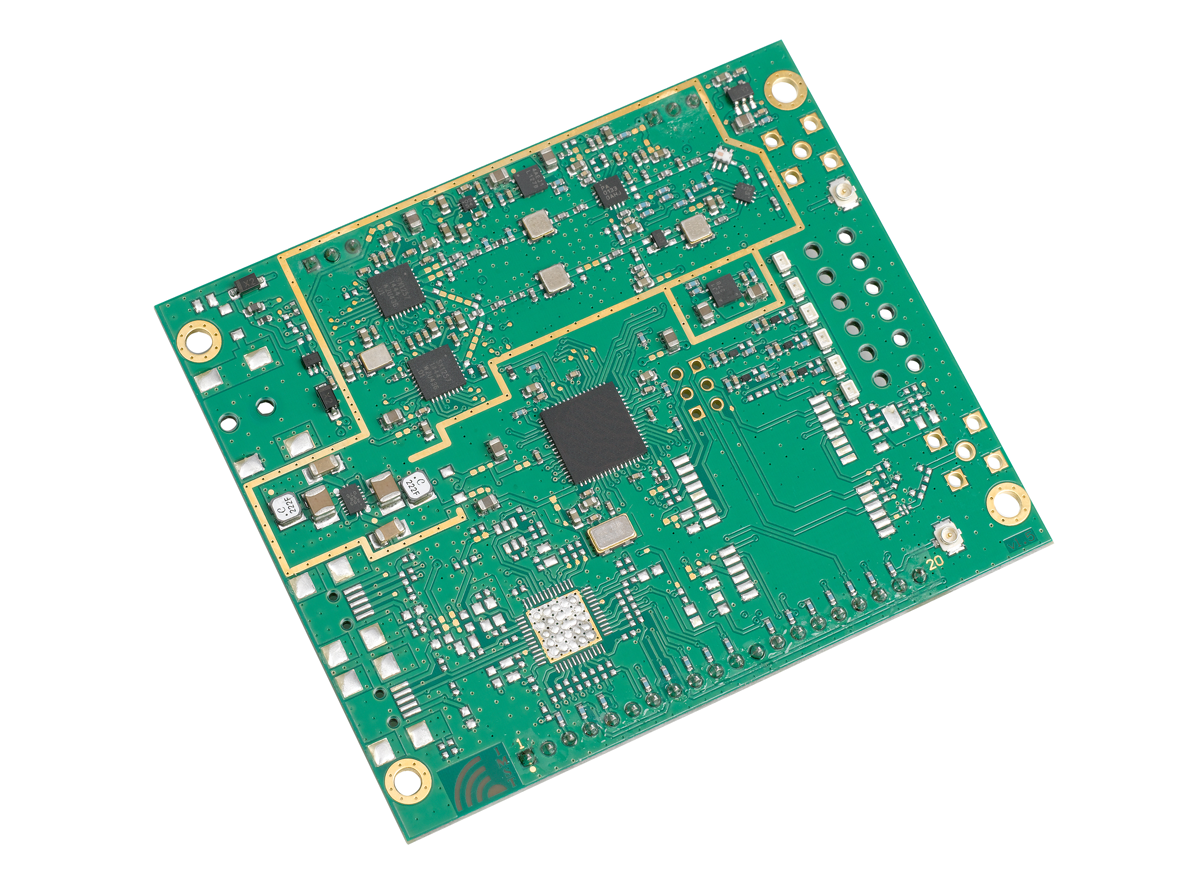
\includegraphics[width=350px]{ic880a-spi}
	\caption{iC880A-SPI - LoRaWAN Concentrator 868 MHz}
	\label{}
\end{figure}

Afin de connecter ce module au Raspberry, un shield tel que le \textit{RPi to iC880a interface} est nécessaire.

\newpage

\subsubsection{Bridge}

Dans notre cas, le bridge fait partie intégrante de la gateway. Sur le schéma dans la \autoref{objectifssysteme}, ce dernier est séparé de la gateway afin de bien représenter le passage de l'utilisation du protocole \textit{LoRa} vers le protocole \textit{MQTT}.
Plus d'informations sont disponibles sur le github suivant : \url{https://github.com/heig-vd-iot2018/infrastructure}

\subsubsection{Network Server}

Ce dernier est divisé en trois parties différentes : Routeur, Broker et Network server.
Plus d'informations sont disponibles sur le github suivant : \url{https://github.com/heig-vd-iot2018/infrastructure}
\subsubsection{Backend}

Le backend est développé en Node.js avec le framework Express. Ce dernier reçoit des informations depuis le network server et traite ces informations avant de pouvoir fournir ces dernières au frontend.
Plus d'informations sont disponibles sur le github suivant : \url{https://github.com/heig-vd-iot2018/back-end}

\subsubsection{Frontend}
Le frontend consiste en la mise en place d'une interface utilisateur permettant de voir les différentes valeurs fournies par les capteurs. Ce dernier a été développé à l'aide des technologies suivantes : \textbf{React}, \textbf{D3} et \textbf{Mapbox.js}.
Plus d'informations sont disponibles sur le github suivant : \url{https://github.com/heig-vd-iot2018/front-end}

%------------------------ Biens a protéger ---------------------------------
\newpage
\subsection{Biens nécessitants une protections}

Les biens principaux à sécuriser sont toutes les données qui peuvent contenir des informations métier ou clients. Par exemple, les données transmises par les capteurs ne doivent pas être lisibles par des personnes non-autorisées au cours de leur trajet.

Les biens concernés par cette protection sont les suivants :

\begin{itemize}
\item[•] Les données transmises par les capteurs
\begin{itemize}
\item Identité
\item Géo-localisation
\item Données environnementales
\end{itemize}
\item[•] Les données utilisateurs
\begin{itemize}
\item Adresses e-mails \footnote{Afin d'éviter toute réutilisation pour du phishing ou du spamming de masse.}
\item Rôles des utilisateurs \footnote{Pour éviter les vols de session ciblés.}
\item Mots de passe \footnote{Les raisons sont évidentes et de plus ces mots de passe pourraient être ajouté à des listes de brute-force.}
\end{itemize}
\item[•] Le fonctionnement de l'application
\item[•] Les appareils et éléments physiques qui font tourner l'architecture
\end{itemize}

Ces biens doivent être protégés à tous les niveaux et à tous les endroits où elles sont susceptibles d'apparaitre (e.g. des capteurs à la gateway mais aussi de la gateway au serveur d'application).

%------------------------ Périmètre sécurisation ---------------------------
\subsection{Périmètre de sécurisation}

Dans ce projet, la sécurité doit être analysée sur chacun des éléments qui composent l'architecture mais aussi sur les liens entre eux. Il n'y a aucune zone considérée comme "sûre de base", il faut donc penser à tous les éléments suivants :

\begin{itemize}
\item[•] Sécurisation des connexions aux éléments physiques.
\item[•] Sécurisation des trames à l'intérieur du protocole LoRa.
\item[•] Sécurisation des accès au back-end et au front-end.
\item[•] Sécurisation de toutes les communications MQTT.
\item[•] Sécurisation des éléments hébergeant les différents éléments de l'infrastructure.
\item[•] Sécurisation et gestion des version pour les technologies, langages et librairies utilisées.
\end{itemize}

%------------------------ Diagramme des flux -------------------------------
\subsection{Diagramme des flux}
\label{ssec:diagramme}

%------------------------ Sources de menaces -------------------------------
\clearpage
\section{Sources de menaces}

Différentes sources de menaces existent autour des applications web mais aussi autour du monde de l'\emph{Internet des objets}. Dans le cadre de notre projet nous retrouvons les catégories de menaces décrites ci-dessous :

\begin{itemize}

\item[•] \textbf{Étudiants kleptomanes}

\begin{tabular}{lp{13cm}}
Motivation: & Gagner un capteur, une gateway, une Raspberry Pi gratuite \\
Cible: & Le matériel \\
Probabilité: & Haute \\
\end{tabular}
\medskip

\item[•] \textbf{Hacker, script-kiddies}

\begin{tabular}{lp{13cm}}
Motivation: & S'amuser, s'entraîner, le faire pour la reconnaissance \\
Cible: & Tout ce qui peut être visé et qui entre dans ses compétences \\
Probabilité: & Moyenne \\
\end{tabular}
\medskip

\item[•] \textbf{Éventuels concurrents}

\begin{tabular}{lp{13cm}}
Motivation: & Récupération des particularités de l'application (espionnage industriel) \\
Cible: & Le fonctionnement de l'application \\
Probabilité: & Moyenne \\
\end{tabular}
\medskip

\item[•] \textbf{Cybercriminels}

\begin{tabular}{lp{13cm}}
Motivation: & Récupérer des adresses mails (spaming) et mots de passe, se servir de l'application web comme passerelle vers son site malveillant ou pour répandre un virus \\
Cible: & Les données des utilisateurs, l'accès à la partie web \\
Probabilité: & Faible \\
\end{tabular}
\medskip

\item[•] \textbf{Organisation étatique}

\begin{tabular}{lp{13cm}}
Motivation: & Récolter des données, espionner \\
Cible: & Toute l'application \\
Probabilité: & Presque nulle \\
\end{tabular}
\medskip

\end{itemize}

%------------------------ Début scénarios ----------------------------------
\section{Scénarios d'attaque}
\label{sec:scenarios}

Dans les sections ci-dessous, différents scénarios d'attaque sont listés et analysé en détails. Pour chacun d'eux, les failles qui existaient dans le projet ont été listées et analysées. Toutes les contre-mesures appliquée pour les corriger sont détaillées dans la \autoref{sec:contremesures}. Dans la \hyperref[sec:conclusion]{conclusion}, vous retrouverez toutes les listes des failles existantes, absente, corrigées ou exploitables.

Un scénario d'attaque correspond à une marche à suivre qu'un attaquant souhaitant attaquer le système suivrait pour arriver à ses fins. Celui-ci est généralement élaboré par un ingénieur sécurité s'étant mis à la place d'un attaquant. Cet exercice permet de mieux comprendre les vecteurs d'attaque, l'impact, les motivations et les potentielles cibles d'un individu malveillant. Ces scénarios ne représentent pas les failles sécuritaires à proprement parlé, mais les motivations générales qu'un attaquant peut avoir pour attaquer le système.

Chacun des chapitres ci-dessous reprend donc un scénario d'attaque ainsi que les failles qui lui sont associées. Avec chaque scénario, se trouve un résumé des enjeux et la liste des failles ainsi que la manière dont elles peuvent être exploitées.

\subsection{Vol d'informations dans la base de données}

\emph{Ce scénario concerne principalement les groupes front-end et back-end}.
\medskip

Comme dans la plupart des applications web et des projets de cette envergure, le groupe \emph{back-end} a mis en place une base de données. Celle-ci est évidemment une cible privilégiée pour les attaquants car elle contient toutes les informations métiers et celles nécessaires à la plateforme web.
\medskip

\renewcommand{\arraystretch}{1.6}
\begin{tabular}{@{}p{4cm}p{12cm}}
\textbf{Scénario:} &  \\
\textbf{Impact:} & Haut \\
\textbf{Source de menace: } & Concurrents, script kiddies, hackers et cybercriminels \\
\textbf{Motivation:} & La gloire (script kiddies, hackers)

L'argent (cybercriminels)

L'espionnage industriel (concurrents) \\
\textbf{Cible:} & Données utilisateurs et données métier \\
\textbf{Contrôles:} & Caché le contenu de la base de données

Sécuriser son accès
\end{tabular}
\renewcommand{\arraystretch}{1}

\subsubsection{Injections SQL}

\subsubsection{Lisibilité du contenu sensible}

\subsubsection{Gestion d'accès}

%\begin{itemize}
%\item Injections SQL
%\item Conservation des mots de passe dans la DB
%\item Accès direct à la base de données (port 3306 ouvert)
%\item Gestion version, droits utilisateurs, built-in fonctions
%\end{itemize}

\clearpage
\subsection{Contournement d'authentification}

\emph{Ce scénario concerne principalement les groupes front-end et back-end}.
\medskip

Comme précisé dans notre diagramme des flux (\autoref{ssec:diagramme}), nous voyons qu'il existe plusieurs rôles communiquant avec le back-end.

\begin{enumerate}
\item Les administrateurs
\item Les utilisateurs normaux
\item Les capteurs
\end{enumerate}

Ceux-ci disposent bien évidemment de possibilités différentes dans le cadre du projet. Évidemment cette séparation des pouvoirs est importante et les cloisonnement des rôles est primordial afin de limiter au maximum les abus. Un utilisateur normal ayant la possibilité d'abuser le système pour devenir administrateur, peut représenter un grand risque pour la plateforme. Tous les autres cas de changement illicite de rôle sont tout aussi risqués et il est nécessaire de mettre en place des protections contre ce genre de motivations.
\medskip

\renewcommand{\arraystretch}{1.6}
\begin{tabular}{@{}p{4cm}p{12cm}}
\textbf{Scénario:} &  Jean-Kevin, un script kiddy entreprenant, souhaite montré à ses copains ses progrès en informatique. Pour cela, il prend pour cible un projet sur lequel travaille activement un de ces collègues étudiant à la HEIG-VD. Il veut montrer qu'il peut se connecter en tant qu'administrateur sans connaître le
mot de passe. Il arrive à ses fins en se connectant au compte d'un
administrateur qui n'était pas protéger par un mot de passe fort et
peut disposer à sa guise de l'application.\\
\textbf{Impact:} & Haut \\
\textbf{Source de menace: } & Script kiddies, hackers \\
\textbf{Motivation:} & La gloire (script kiddies)

Nuire à l'application et aux utilisateurs (hackers)\\
\textbf{Cible:} & Données et fonctionnement de l'application \\
\textbf{Contrôles:} & Protéger la session ouverte contre des vols de sessions externes

Empêcher l'utilisateur de faire malgré lui des actions dans sa session

Protéger correctement les sessions avec des mots de passe forts
\end{tabular}
\renewcommand{\arraystretch}{1}

\subsubsection{Cross-site scripting}

\subsubsection{Brute-force du système de login}

\subsubsection{Actions involontaires de l'utilisateur}

\subsubsection{Contrôles d'accès}

\subsubsection{Durée de vie de la session}

%\begin{itemize}
%\item XSS
%\item Brute-force login
%\item CSRF et autres
%\item Contrôle d'accès
%\item Durée de vie de session
%\end{itemize}

\subsection{Récupération passive d'information}

\emph{Ce scénario concerne principalement le groupe infrastructure.}
\medskip

Souvent, on imagine un hacker pénétrant le système et réalisant des \textbf{actions} sur ce dernier. Ne considérer que ce pan de la sécurité est une grave méprise. Rappelons le triangle suivant :

\begin{figure}[h]
\begin{center}
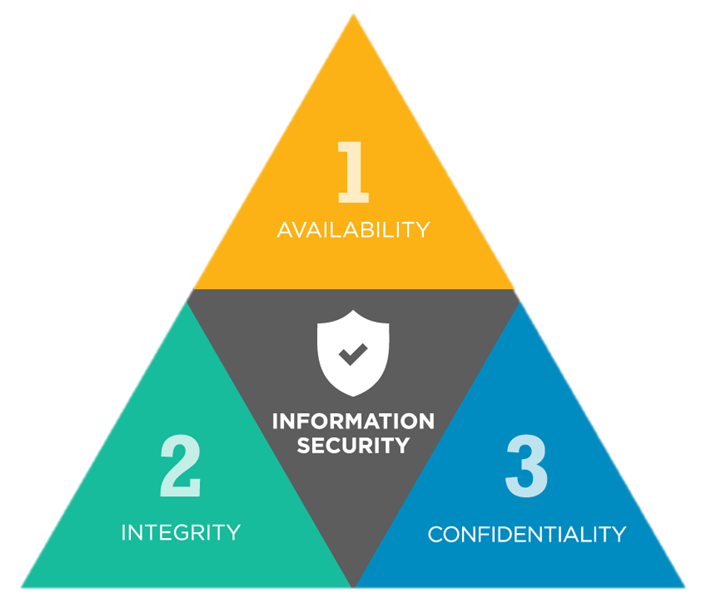
\includegraphics[width=.6\textwidth]{CAI.png}
\caption{Principes essentiels de la sécurité informatique}
\end{center}
\end{figure}

La confidentialité peut en effet être mise à mal sans même une action directe sur les données. L'interception peut permettre la lecture de ces dernières et si l'information n'est pas obfusquée, on peut récupérer des données sans le consentement des parties et donc mettre à mal la sécurité de l'information. Il est donc primordial de protéger les données dans leur transmission surtout sur des médiums partagés.
\medskip

\renewcommand{\arraystretch}{1.6}
\begin{tabular}{@{}p{4cm}p{12cm}}
\textbf{Scénario:} &  Les concurrents directs de notre application cherche à obtenir un maximum de données afin de proposer un service plus précis et exhaustif que le notre. Pour arriver à leur fins ils décident d'écouter le trafic généré par nos capteurs à l'intérieur de l'école. Si le trafic n'est pas chiffré, les concurrents peuvent l'utiliser de manière illicite dans leur alternative.\\
\textbf{Impact:} & Haut \\
\textbf{Source de menace: } & Hackers, concurrents et cybercriminels \\
\textbf{Motivation:} & Tremplin vers une plus grosse attaque (hackers)

L'argent (cybercriminels)

Nuire à notre image, voler des données (concurrents)\\
\textbf{Cible:} & Les données utilisateurs et métier \\
\textbf{Contrôles:} & Éviter que l'application ne fournisse des données sur elle-même ou sur les utilisateurs

Protéger les communications entre les éléments du système
\end{tabular}
\renewcommand{\arraystretch}{1}

\subsubsection{Communications authentifiées et chiffrées (TLS)}

\subsubsection{Chiffrement des trames LoRa}

\subsubsection{Messages d'erreur révélant des informations}

%\begin{itemize}
%\item SSL/TLS
%\item Chiffrement des trames LoRa
%\item Messages d'erreurs
%\end{itemize}

\subsection{Utilisation frauduleuse du matériel}

\begin{itemize}
\item Protection modification du hardware (signature, tamper-proofing)
\item Contrôle d'accès physique
\item Association sécurisée
\end{itemize}

\subsection{Altération des données}

\begin{itemize}
\item Signature des trames LoRa
\item \emph{Man in the middle}
\item Association sécurisée (capteur - serveur)
\end{itemize}

\subsection{Altération du fonctionnement de l'application}

\begin{itemize}
\item Dos
\item Buffer-overflow
\item Trafic jamming
\item Système hébergeur et services pas à jour
\end{itemize}

%------------------------ Contremesures ------------------------------------
\section{Contre-mesures}
\label{sec:contremesures}
\subsection{Integrité des trames}
Afin de garantir l'intégrité des données envoyées sur le réseau LoRa, un contrôle d'intégrité de type CRC32 peut être effectué à l'instar du type de contrôle effectué lors de communications Wifi. Cette somme de contrôle serait mise à la suite des données envoyées et le tout pourrait être chiffré, par exemple avec AES dont la clé serait connue du capteur et de la gateway.

Une fois la trame reçue par la gateway, ou par le capteur, elle serait déchiffrée et le CRC32 contrôlé afin d'assurer l'intégrité de la trame reçue.

\subsection{Association sécurisée lora}

\subsection{DDoS}
Afin d'éviter toute attaque du type déni de service, il serait envisageable d'effectuer un contrôle sur les ip se connectant au backend par exemple afin de limiter ou bloquer l'accès de cette dernière au backend si un certain seuil de requêtes par secondes ou minutes est atteint. De plus, il serait possible de mettre les différents serveurs (network server) en liste blanche. Ceci permettrait que seul les gateway et serveurs authorisés puissent se connecter au backend pour pousser des donnés, mitigeant ainsi le risque de DDoS.

En ce qui concerne le frontend, seul un utilisateur authentifié peut accèder aux données. On pourrait filtrer les requêtes ICMP afin d'éviter une attaque de type \textit{smurt attack}. Afin d'éviter une attaque de type \textit{SYN Flood}, on pourrait limiter dans le temps le nombre de requêtes effectuées par un certain client authentifié.

Il serait possible d'héberger le backend sur un fournisseur IaaS afin de permettre un \textit{autoscaling} lorsque le serveur est surchargé. Toutefois, cette solution serait inefficace si l'attaque par DDoS est de grande envergure.

\subsection{Buffer Overflow}

\subsection{systèmes pas à jour}
Si l'infrastructure est hébergée sur un fournisseur IaaS, les mises à jour du système sont à la charge du développeur. Si un service PaaS est utilisé, ces mises à jour sont à la charge du fournisseur de services.

Mettre à jour les applications utilisées ainsi que les systèmes d'exploitations doivent être régulièrement mis à jour afin de contrer les vulnérabilités découvertes et patchées.

\subsection{Protection physique}
L'accès aux différents modules (gateway et senseurs) doivent être protégés afin d'éviter à une tierce partie d'accèder au firmware ou programmes qui tournent sur ces derniers. En effet, si des clés de chiffrement sont disponible sur ces modules afin de chiffrer les trames envoyées entre les senseurs et les gateway, il faut s'assurer que l'accès à cette information est protégé.

Il serait envisageable d'enfermer ces modules dans des armoires techniques fermées à clef afin d'en limiter l'accès.

\subsection{fuse protection}
Ces "protection fuse" peuvent être de type logiciel ou matériel. Ils permettent d'éviter que les éléments de la mémoire soient lus, et par conséquent, sont de plus en plus installés dans les chips de nos jours. Cette protection est mise en place, par exemple, en configurant certains bits dans le chip or en fusionnant les lignes de contrôle correspondantes. Ces \textit{fuse} ne sont pas toujours résistants à différentes techniques de manipulation spécifiques. Ces \textit{Fuse bits} qui sont configurés peuvent être remis à 0 par une injection par laser. Une fois que ces \textit{fuse} sont remis à 0, l'analyse du système (lecture des informations) peut continuer. Une contremesure efficace est un maillage de connecteurs qui est placé autour du chip et éléctriquement connecté à ce dernier. Si le chip est ouvert ou attaqué physiquement, ce maillage est détruit ce qui résulte en la destruction du chip, rendant impossible la récupération des informations (voir \autoref{laser}).

\begin{figure}[!h]
	\centering
	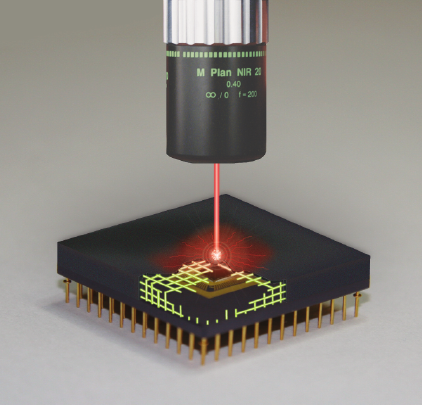
\includegraphics[width=250px]{laserattack.png}
	\caption{Protection anti-modification par maillage}
	\label{laser}
\end{figure}

source : \url{https://www.aisec.fraunhofer.de/content/dam/aisec/Dokumente/Publikationen/Studien_TechReports/englisch/Whitepaper_ProductProtection.pdf}

\newpage

%------------------------ Conclusion ---------------------------------------
\section{Conclusion}
\label{sec:conclusion}

%------------------------ Sources ------------------------------------------
\section{Sources}
\label{sec:sources}

\end{document}
